\documentclass[12pt]{article}
\usepackage{graphicx} % Required for inserting images
\usepackage{float}
\usepackage{listings}
\usepackage[dvipsnames]{xcolor}
\usepackage{geometry}
\usepackage[UTF8]{ctex}
\usepackage{amsmath}
\usepackage{amssymb}

\title{Pre-lecture Problems for Lecture 6:\\ Branch \& Bound and Heuristic Algorithms}
\author{B10705034 資管三\ 許文鑫}
\geometry{a4paper,scale=0.8}
\begin{document}
\maketitle
\begin{enumerate}
      \item [3.] (10 points; 5 points each) Consider the following IP
            \begin{align*}
                  \text{max }  & 3x_1 + 5x_2                                 \\
                  \text{s.t. } & x_1 + 3x_2 \leq 8                           \\
                               & 2x_1 + 4x_2 \leq 15                         \\
                               & x_i \in \mathbb{Z}_+ \quad \forall i = 1, 2
            \end{align*}
            \begin{enumerate}
                  \item Use the branch-and-bound algorithm to solve the IP.\\
                        \textbf{Ans. }
                        We can first solve the LP relaxation of the problem:
                        Solve the LP relaxation:
                        \begin{align*}
                              \text{max }  & 3x_1 + 5x_2                       \\
                              \text{s.t. } & x_1 + 3x_2 \leq 8                 \\
                                           & 2x_1 + 4x_2 \leq 15               \\
                                           & x_i \geq 0 \quad \forall i = 1, 2
                        \end{align*}
                        We can get the optimal solution $(x_1, x_2) = (7.5, 0)$, and the optimal value is $22.5$.\\
                        Then we can branch on the variable $x_1$.
                        \begin{figure}[H]
                              \centering
                              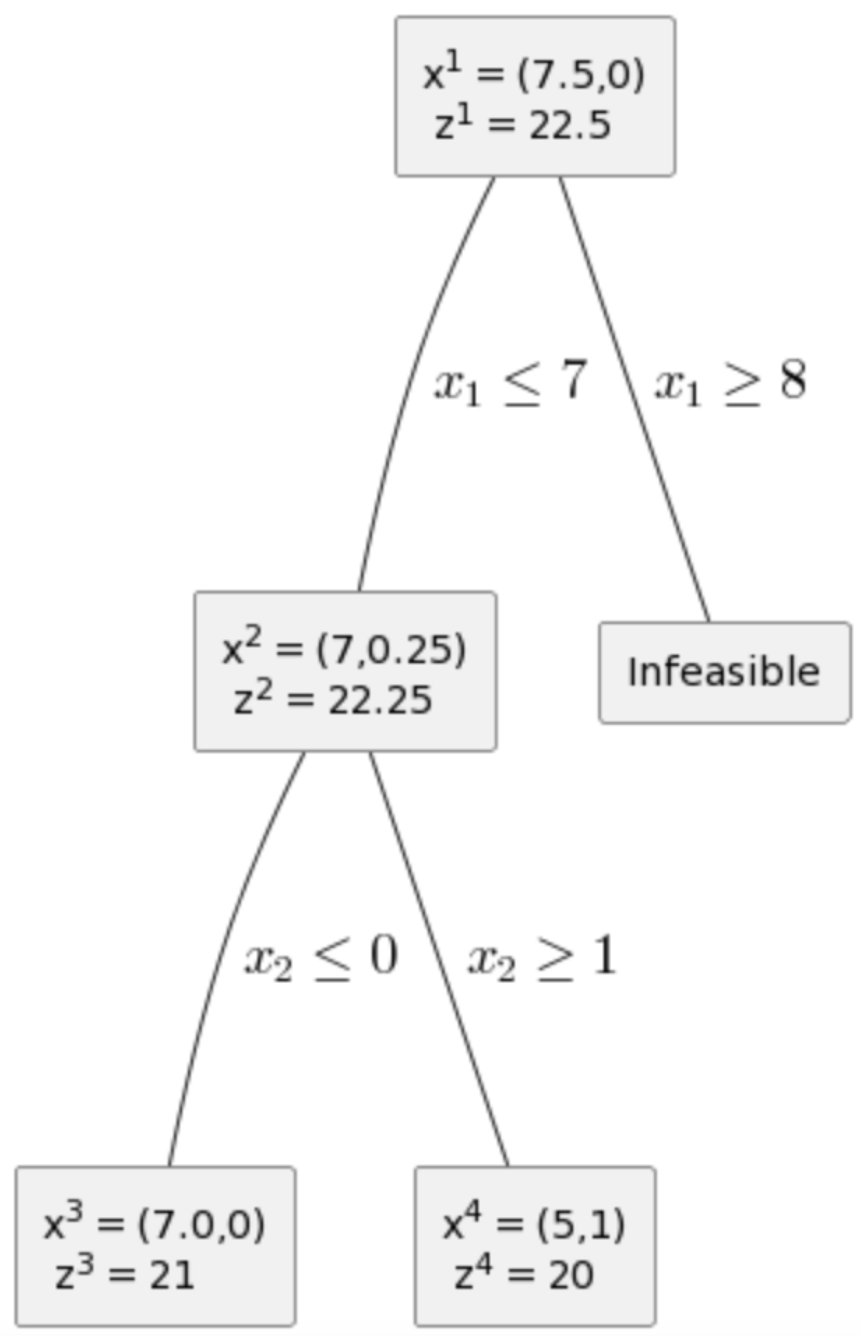
\includegraphics[scale=0.4]{sol.png}
                        \end{figure}
                        The optimal solution is $(x_1, x_2) = (7, 0)$, and the optimal value is $21$.
                  \item Use the following two-step heuristic algorithm to solve the IP: First solve the linear relaxation to obtain an LR-optimal solution $(x_1,x_2)$, and then report $(\lfloor x_1\rfloor,\lfloor x_2\rfloor)$ as an IP-feasible solution. Find the solution reported by the heuristic algorithm. Moreover, calculate the optimality gap by comparing the heuristic solution and the LR-optimal solution. Please note that $(x_1,x_2)$ may be fractional in the LR-optimal solution, but $(\lfloor x_1 \rfloor,\lfloor x_2\rfloor)$ must be integers when reported by the heuristic algorithm.\\
                        \textbf{Ans. } The LR-optimal solution is solved in (a.) which is  $(x_1, x_2) = (7.5, 0)$, and the optimal value is $22.5$. The heuristic solution is $(\lfloor x_1 \rfloor, \lfloor x_2 \rfloor) = (7, 0)$, and the optimal value is $21$. \\
                        The absolute error is $22.5 - 21 = 1.5$.\\
                        The percentage error is $\frac{1.5}{22.5} = 6.67\%$.
            \end{enumerate}
\end{enumerate}
\end{document}